%----------------------------------------------------------------------------
\chapter{Evaluation}\label{chap:evaluation}
%----------------------------------------------------------------------------
\todo[inline]{About 6--8 pages. Criterion E (0--8): full marks require an evaluation beyond small examples, including scalability and robustness measurements that show the system holds up in an industrial setting. Criterion D/2 penalises results whose correctness cannot be checked, so report setup, versions, and repetitions.}

\section{Research questions}
\begin{rqlist}
  \item\label{rq:correct} TODO Does the approach handle the running example and the cases in \cref{chap:intro} correctly?
  \item\label{rq:scale} TODO How do time and resource use grow with input size?
  \item\label{rq:robust} TODO How does the system behave under faults, adversarial input, or load spikes?
\end{rqlist}

\section{Setup}
TODO Hardware, software versions, datasets or workload generators, number of repetitions, and how to rerun the measurements from the repository.

\section{Correctness (RQ1)}
TODO

\section{Scalability (RQ2)}
TODO Describe \cref{fig:scalability}: what grows, how fast, and where the limit is.

\begin{figure}[!ht]
  \centering
  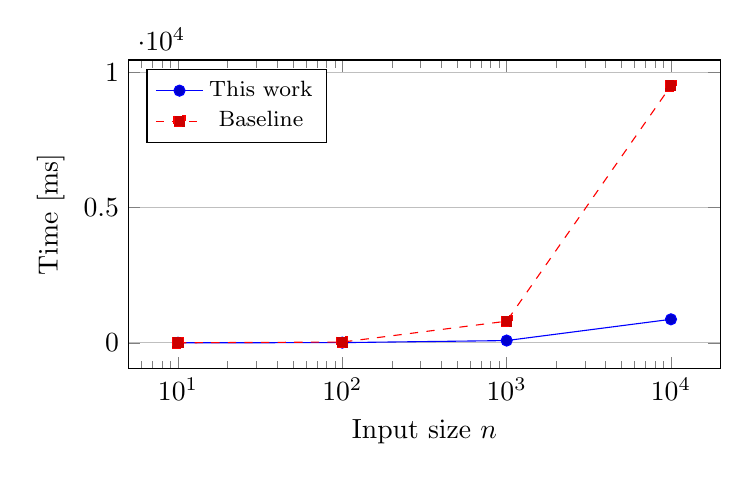
\begin{tikzpicture}
    \begin{axis}[
        width=0.75\linewidth, height=55mm,
        xlabel={Input size $n$}, ylabel={Time [ms]},
        xmode=log, log basis x=10, ymajorgrids,
        legend pos=north west, legend style={font=\footnotesize}]
      \addplot+[mark=*, error bars/.cd, y dir=both, y explicit]
        coordinates {(10,2) +- (0,0.3) (100,9) +- (0,1) (1000,85) +- (0,6) (10000,870) +- (0,40)};
      \addlegendentry{This work}
      \addplot+[mark=square*, dashed]
        coordinates {(10,3) (100,30) (1000,800) (10000,9500)};
      \addlegendentry{Baseline}
    \end{axis}
  \end{tikzpicture}
  \caption{Scalability: mean of TODO runs, error bars show one standard deviation. Placeholder data, replace with your measurements.}
  \label{fig:scalability}
\end{figure}

\section{Robustness (RQ3)}
TODO

\section{Threats to validity}
TODO What could make the results wrong or not generalise, and what you did about each.
